\graphicspath{{/Users/emiliendurif/Documents/prepa/sujets/TP_simulation/ericc3/}}

\question{
\begin{enumerate}
\item Copier le dossier "modele$\_$simscape" sur votre espace perso.
\item Placer le chemin d'acc�s de ce dossier dans la barre d'adresse Matlab.
\item Dans Matlab ouvrir le fichier "ericc3$\_$DataFile.m" et l'ex�cuter. On note dans le workspace la cr�ation d'un objet appel� smiData qui contient l'ensemble des variables m�caniques n�cessaires au calcul.
\item Lancer Simulink et ouvrir le fichier ericc3$\_$simmechanics.slx.
\item Ex�cuter le programme et observer le r�sultat de la simulation. 
\end{enumerate}
}

\question{Compl�ter la chaine fonctionnelle d�crivant la chaine cin�matique "axe de lacet".}

\begin{center}
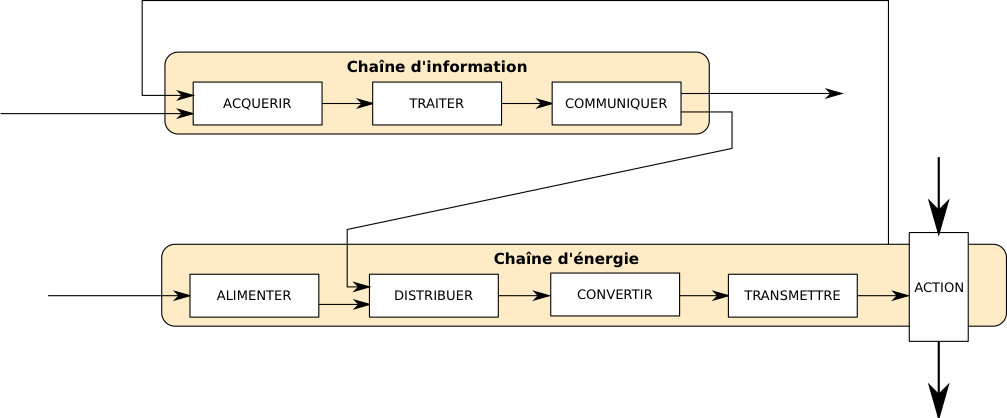
\includegraphics[width=1.0\textwidth]{images/chaine_fonctionnelle.png}
\end{center}


\question{Dans Simulink, r�aliser le sch�ma �lectrique de la motorisation du robot sans la conversion �lectrom�canique.}

\begin{center}
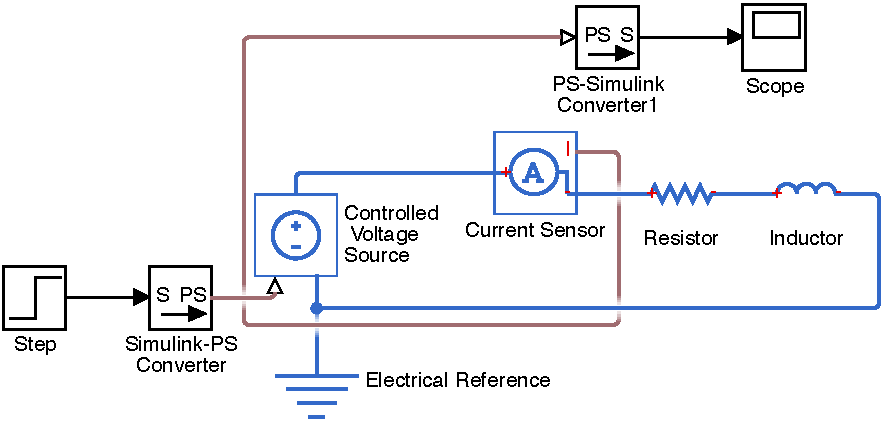
\includegraphics[width=0.9\textwidth]{images/ericc_mcc_elec.pdf}
\end{center}

\question{Dans Simulink, r�aliser le sch�ma m�canique de la motorisation du robot sans la conversion �lectrom�canique.}

\begin{center}
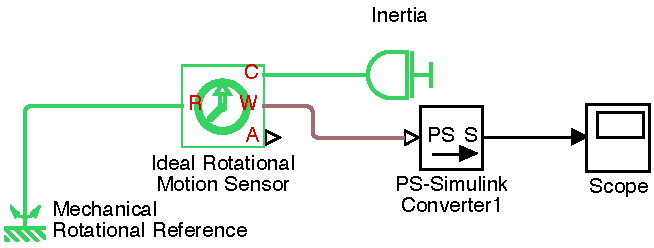
\includegraphics[width=0.9\textwidth]{images/ericc_mcc_meca.pdf}
\end{center}

\question{Raccorder les deux sch�mas �lectrique et m�canique d�finis pr�c�demment � l'aide du bloc de conversion �lectrom�canique.}

\question{R�aliser la simulation consistant � imposer un �chelon de tension au moteur et � visualiser le r�ponse en vitesse de rotation du moteur.}



\question{A l'aide des �quations \ref{eq_meca}, \ref{eq_elec}, \ref{eq_elec_meca1} et \ref{eq_elec_meca2}, construire le sch�ma bloc d�crivant la mod�lisation causale du moteur. (On prendra en entr�e $u_m(t)$ et en sortie $\omega_m(t)$}

\begin{center}
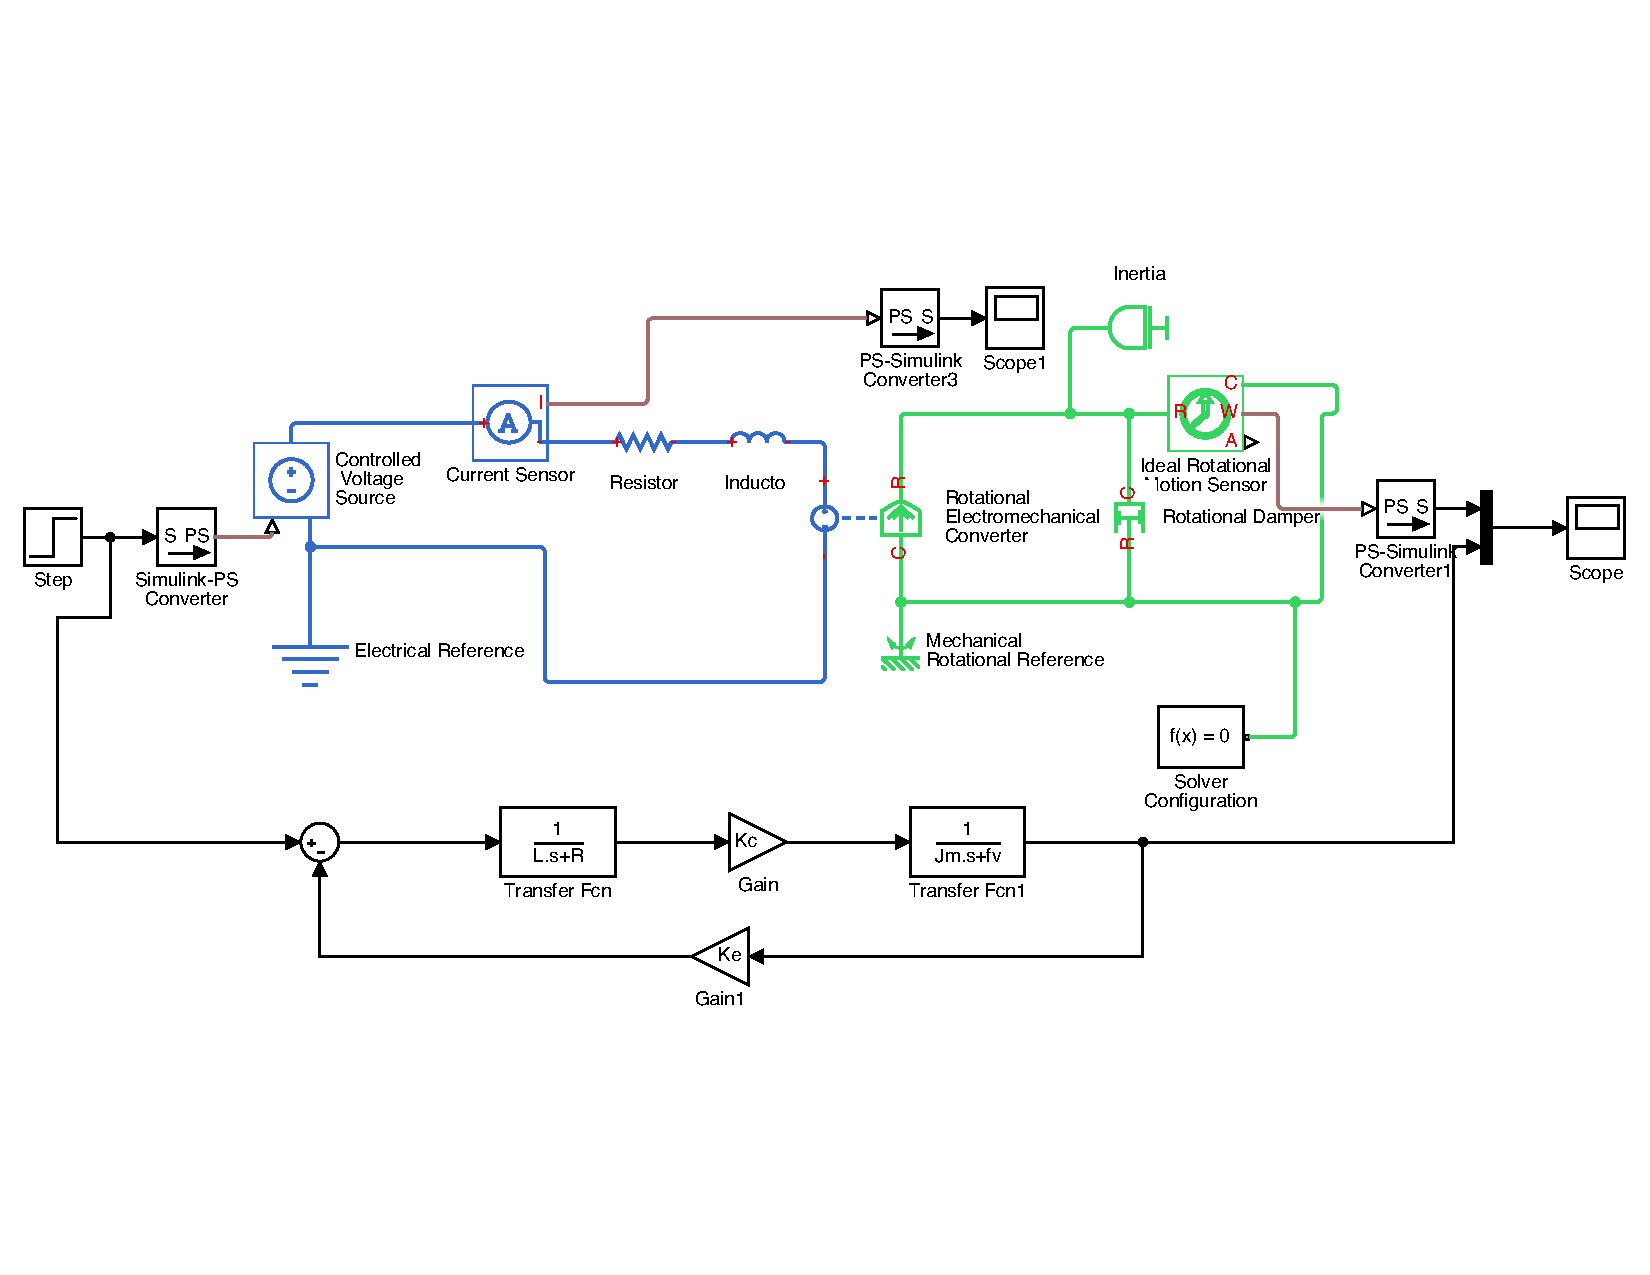
\includegraphics[width=0.9\textwidth]{images/modele_mcc_ericc.pdf}
\end{center}

\question{D�terminer le rapport de r�duction $K_r$ du syst�me.}


\question{Compl�ter le sch�ma bloc "modele$\_$ericc$\_$complet$\_$eleve.slx" pour mod�liser le syst�me asservi en boucle ferm�e. 
}

\begin{center}
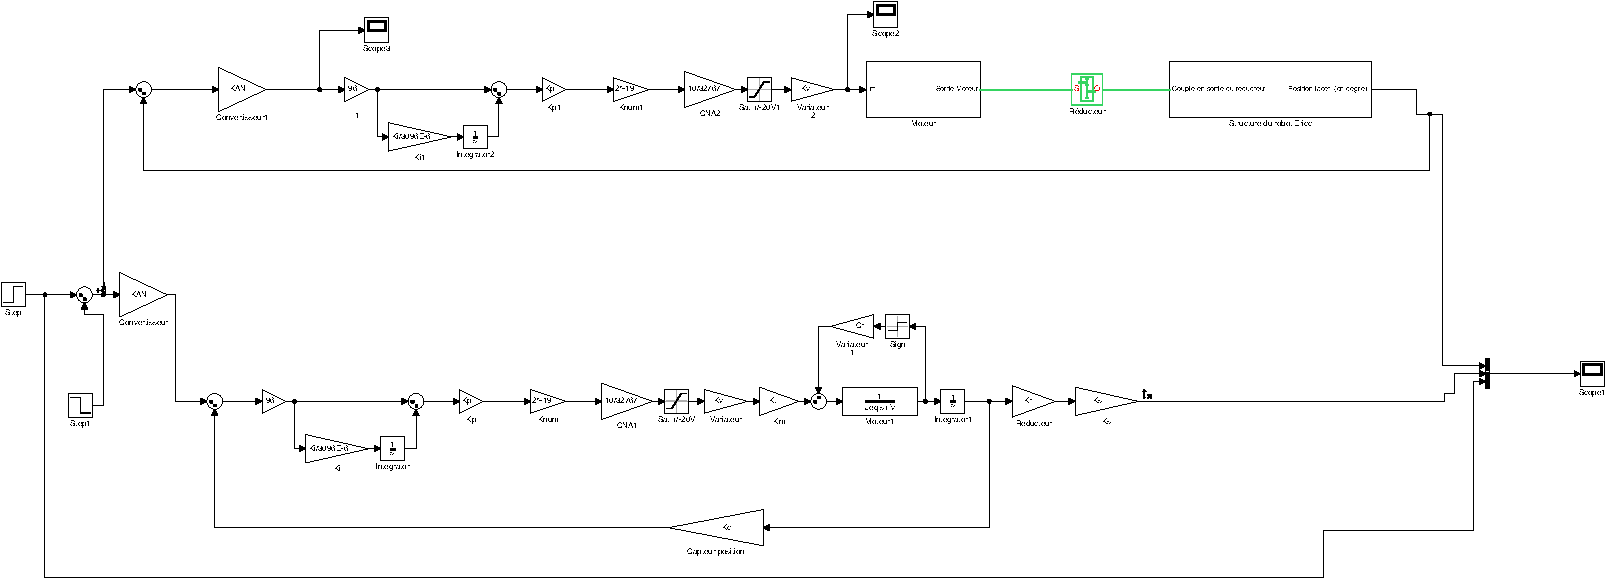
\includegraphics[width=0.9\textwidth]{images/modele_ericc_complet.pdf}
\end{center}